\documentclass{article}
\usepackage{style}

\begin{document}
  \title{FYS1210}
  \author{Robin A. T. Pedersen \and Dawid P. Kuleczko}
  \maketitle
  \tableofcontents

  \section{Forord}
    Dette dokumentet er hovedsaklig skrevet for meg selv i et forsøk på å tvinge hjernen min til å behandle informasjonen inneholdt i pensum.
Kanskje vil det bli noe andre kan bruke hvis de ikke gidder å lese hele læreboka, eller det kan brukes som oppsummering før eksamen?
\\

Se etter feil og si ifra hvis du gidder.


  \section{Uke 3 - Introduksjon}
    Ledere, isolatorer, halvledere, Ohms lov, serie- og parallellkobling, Kirchoff, superposisjon og Thevenin.

\subsection{Serie- og parallellkobling}
\subsubsection{Seriekobling}
TODO

\subsubsection{Parallellkobling}
TODO


\subsection{Kirchhoff}
\subsubsection{Kirchhoffs lov om strømmer}
TODO



\subsubsection{Kirchhoffs lov om spenninger}
TODO



\subsubsection{Spenningsdeler}
Vi ser på tilfellet med to motstander seriekoblet til et batteri.
\\
\begin{circuitikz} \draw
(0,0) to[battery, l=$V_{batteri}$] (0,4)
      -- (4,4)
      to[R, l=$R_2$] (4,2)
      to[R, l=$R_1$] (4,0)
      -- (0,0)
      ;
\end{circuitikz}
\\
Hva er spenningen $V_1$ over motstanden $R_1$?
$$V_1 = \frac{R_1}{R_1 + R_2} \cdot V_{batteri}$$

Du kan tenke på det som dette:
\\
Hvor stor del av kaka tar $R_1$?
sin rettferdige andel: $\frac{R_1}{R_1 + R_2}$
\\
Hvor mye kake er det egentlig? $V_{batteri}$


\subsection{Superposisjon}
Superposisjonsprinsippet brukes til å finne verdier i kretser med mer enn én spenningskilde.
For å finne spenningen rundt en komponent ser man på bidraget fra én spenningskilde om gangen.
Når bidraget fra alle kildene er funnet, legger man det sammen for å få totalverdien.

\subsubsection{Eksempel}
$V_{S1}=\SI{15}{\volt}$,\qquad
$V_{S2}=\SI{3}{\volt}$,\qquad
$R_1=R_2=R_3=\SI{1}{\kilo\ohm}$



\begin{circuitikz} \draw
(0,0) to[battery, l=$V_{S1}$] (0,4)
      to[R, l=$R_2$] (4,4)
      -- (8,4)
      to[R, l=$R_1$] (8,0)
      -- (0,0)
(4,0) to[battery, l=$V_{S2}$] (4,2)
      to[R, l=$R_3$] (4,4)
      ;
\end{circuitikz}
\\
I denne kretsen er det to spenningskilder som begge bidrar til å
skape spenning $V_1$ rundt motstanden $R_1$.



\begin{circuitikz} \draw
(0,0) to[battery, l=$V_{S1}$] (0,4)
      to[R, l=$R_2$] (4,4)
      -- (8,4)
      to[R, l=$R_1$] (8,0)
      -- (0,0)
(4,0) -- (4,2)
      to[R, l=$R_3$] (4,4)
      ;
\end{circuitikz}
\\
Vi later som den ene spenningskilden $V_{S2}$ ikke eksisterer
og regner ut bidraget fra $V_{S1}$.



\begin{circuitikz} \draw
(0,0) to[battery, l=$V_{S1}$] (0,4)
      to[R, l=$R_2$] (4,4)
      to[R, l=$R_{EQ}$] (4,0)
      -- (0,0)
      ;
\end{circuitikz}
\\
Motstandene $R_1$ og $R_3$ danner en parallellkobling som vi kan
betrakte som én motstand $R_{EQ}$.
Siden $R_1$ og $R_3$ er parallellkoblet får man
$R_3$ via den \emph{inverse}.
$$\frac{1}{R_{EQ}} = \frac{1}{R_1} + \frac{1}{R_3}$$
Eller, siden det bare er to motstander, via forenklingen.
$$R_{EQ} = \frac{R_1 \cdot R_3}{R_1 + R_3} = \frac{1\cdot 1}{1+1}=\frac{1}{2}$$
%TODO: enheter



  \section{Uke 4 - Fysikalsk elektronikk}
    Kap.  7, s.203-217 \\
Kap.  9, s.247-279 \\
Kap. 12, s.364-382 \\
Kap. 13, s.389-413 \\
Kap. 15, s.462-500 \\
Kap. 16, s.510-528

\subsection{Thevenins Teorem}
\subsubsection{Last-analyse}
Thevenins teorem er en regneteknikk hvor du kan betrakte noe komplisert som noe enkelt.
Det brukes som regel for å regne på forksjellig last uten å måtte regne ut hele kretsen på nytt.

\begin{circuitikz} \draw
(0,0) -- (0,4)
      node [right=3em,below=3em,anchor=west]
           {\large{\textsc{Komplisert krets}}}
      -- (6,4)
      -- (6,0)
      -- (0,0)
(6,3) to[short, -o] (7,3)
      to[voltmeter] (7,1)
      to[short, o-] (6,1)
      ;
\draw[dashed]
(7,3) -- (8,3)
      to[R, label=$R_L$] (8,1)
      -- (7,1)
      ;
\end{circuitikz}
\\
Alle topolede, lineære nettverk (krets)...
\\\\

\begin{circuitikz} \draw
(0,0) -- (0,4)
      -- (6,4)
      -- (6,0)
      -- (0,0)
(6,3) to[short, -o] (7,3)
      to[voltmeter] (7,1)
      to[short, o-] (6,1)
      -- (1,1)
      to[battery] (1,3)
      node[right=1em,below=2.5em,anchor=west]{$V_{TH}$}
      to[R, label=$R_{TH}$] (6,3)
      ;
\draw[dashed]
(7,3) -- (8,3)
      to[R, label=$R_L$] (8,1)
      -- (7,1)
      ;
\end{circuitikz}
\\
...kan erstattes med en spenningskilde $V_{TH}$ og en motstand $R_{TH}$.
\\\\
$V_{TH}$=Spenningen over polene uten last.\\
$R_{TH}$=Motstand over polene når alle spenningskilder er kortsluttet og alle strømmer brutt.



\subsubsection{Eksempel}
\begin{circuitikz} \draw{}
(0,1) -- (0,0) node[ground]{}
(0,0) to[battery, label=$V_S$] (0,4)
      to[R, label=$R_1$] (4,4)
      to[R, label=$R_2$] (4,2)
      to[R, label=$R_3$] (4,0)
      node[ground]{}
(4,2) -- (8,2)
      to[R, label=$R_L$] (8,0)
      node[ground]{}
      ;
\end{circuitikz}
\\
Denne kretsen kan skrives om til å ligne på beskrivelsen av Thevenin ovenfor.
\\

\begin{circuitikz} \draw{}
(1,1) to[battery, label=$V_S$] (1,3)
      to[R, label=$R_1$] (3,3)
      to[R, label=$R_2$] (5,3)
      to[R, label=$R_3$] (5,1)
      -- (1,1)
(5,3) to[short, -o] (7,3)
(5,1) to[short, -o] (7,1)
(0,0) -- (0,4)
      -- (6,4)
      -- (6,0)
      -- (0,0)
      ;
\draw[dashed]
(7,3) -- (8,3)
      to[R, label=$R_L$] (8,1)
      -- (7,1)
      ;
\end{circuitikz}
\\

Vi regner ut $V_{TH}$:\\
Spenning målt over polene uten last,
tilsvarer å måle spenning rundt $R_3$.\\
(Husk at $R_1$ og $R_2$ står i serie)
$$V_{TH} = V_3 = \frac{R3}{(R_1 + R_2) + R_3} \cdot V_S$$
\\

Vi regner ut $R_{TH}$:\\
Motstand over polene når spenningskilder er kortsluttet,
blir som å betrakte kretsen som en parallellkobling.
$$R_{TH} = \frac{(R_1 + R_2)R_3}{(R_1 + R_2) + R_3}$$


\subsubsection{Nortons Teorem}
TODO


\subsection{Spenningskilder - Batterier}
\subsubsection{Virkemåte}
TODO

\subsubsection{Maksimal effektoverføring}
TODO


\subsection{Fysikalsk elektronikk}
Etter Niels Bohrr atommodell ligger elektroner i skall rundt atomkjernen.
Disse skallene kalles bånd.

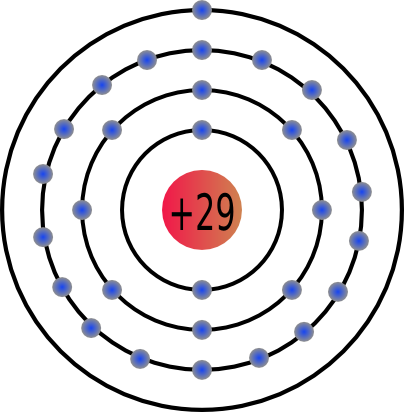
\includegraphics[width=0.25\textwidth]{./img/bohr-Cu}
\\
Kobberatom med 29 protoner og 29 elektroner.\\
Skall 1: 2 elektroner \\
Skall 2: 8 elektroner \\
Skall 3: 18 elektroner \\
Skall 4: 1 elektron
\\
Det ytterste elektronet har en svakere binding til kjernen.

TODO


\subsection{Doping}
TODO


\subsection{Vekselstrøm}
TODO


\subsection{DC-Offset}
TODO


\subsection{Pulser}
TODO



  \section{Uke 5 - Kondensatorer}
    Kap. 12, s.364-382 \\
Kap. 13, s.389-413 \\
Kap. 15, s.462-500 \\
Kap. 16, s.510-528 \\
Kap. 17, s.533-564 \\
Kap. 18, s.574-605

\subsection{Kondensatorer}
\subsubsection{Beskrivelse}
En kondensator (engelsk: capasitor)
er en av de mest fundamentale kompenentene vi bruker.
Dens funksjon er å lagre elektrisk ladning.
De brukes bl.a. til lokal energilagring (som et lite batteri),
dempe brå forandring av spenning (for å beskytte sårbare komponenter)
og signalfiltrering.



\subsubsection{Virkemåte og symbol}
En kondensator består av to ledende plater
med et isolerende materiale (et dielektrisk) i mellom.
\\
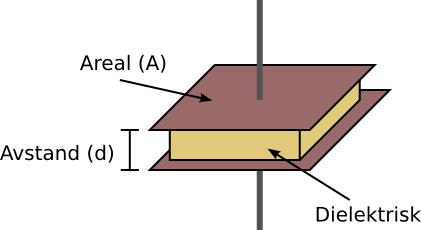
\includegraphics[width=0.5\textwidth]{./img/kondensator-basic}
\\\\
\emph{Symbolet} for en kondensator gjenspeiler oppbygningen.
\\
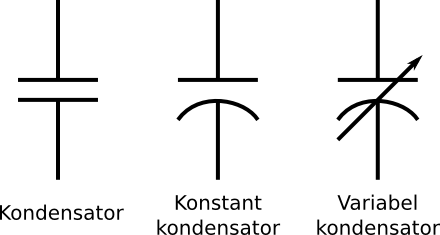
\includegraphics[width=0.5\textwidth]{./img/kondensator-symboler}
\\
\paragraph{Spenning} \mbox{} \\
Når en kondensator kobles til en spenningskilde
vil det gå strøm gjennom kretsen.
Elektronene strømmer \emph{mot} den ene siden av kondensatoren,
og \emph{fra} den andre siden.
\\
Men strømmen blir blokkert av dielektrikumet
og går ikke gjennom kondensatoren.
Istedenfor samler elektronene seg på den ene siden,
og det blir en mangel på elektroner på andre siden.
\\
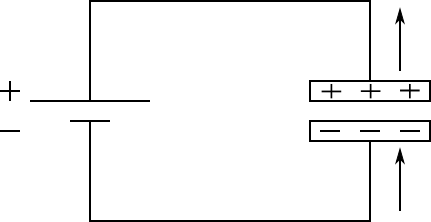
\includegraphics[width=0.5\textwidth]{./img/kondensator-ladning}
\\
Man kan tenke på det som om det går to strømmer.
En fra negativ pol til kondensatoren.
Og en fra kondensatoren mot positiv pol.
\\\\
Nå er det negative ladninger på den ene siden,
og positive på den andre.
Det vil si at vi har en spenning over kondensatoren.



\subsubsection{Formler og enheter}
Kapasitet(ladning), kapasitet(areal), serie, parallell \\
TODO


\subsection{Kondensatorer i kretser}
\subsubsection{DC-kretser}
Impossible for current [...] across cap (in DC?) \\
TODO

\subsubsection{AC-kretser}
Faseforskyvning \\
Reaktanse \\
Decoupling caps \\
TODO

\subsubsection{RC-kretser}
Impedans \\
TODO


\subsection{Frekvensfilter}
\paragraph{Lavpass} \mbox{} \\
TODO



\paragraph{Høypass} \mbox{} \\
TODO



\paragraph{Eksempel} \mbox{} \\
TODO


\subsection{Dioder}
TODO



  \section{Uke 6 - Dioder}
    Kap. 17, s.533-564
Kap. 18, s.574-605

\subsection{Kovalente bindinger}
\subsubsection{Diamantstruktur}
Vi vet allerede at halvledere har 4 elektroner i valensbåndet.
Etter oktettregelen ønsker disse atomene
å fullføre sitt ytterste skall med 8 elektroner.
For å oppnå dette, danner de kovalente bindinger (elektronparbininger)
med andre atomer.
\\
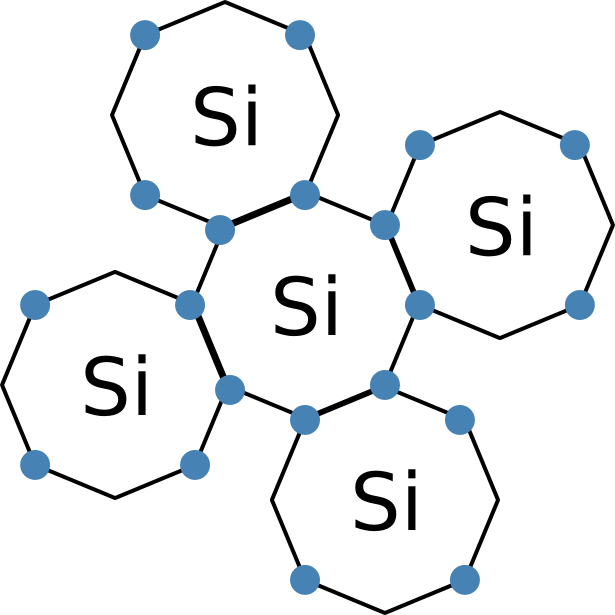
\includegraphics[width=0.5\textwidth]{./img/krystall.png}
\\
Silisiumatmoer danner en krystallstruktur.

\subsubsection{Ledning i rene halvledere}
Ved tilført energi (varme eller lys) kan elektronene løsrives
fra valensbåndet og bevege seg fritt i ledningsbåndet.
\\
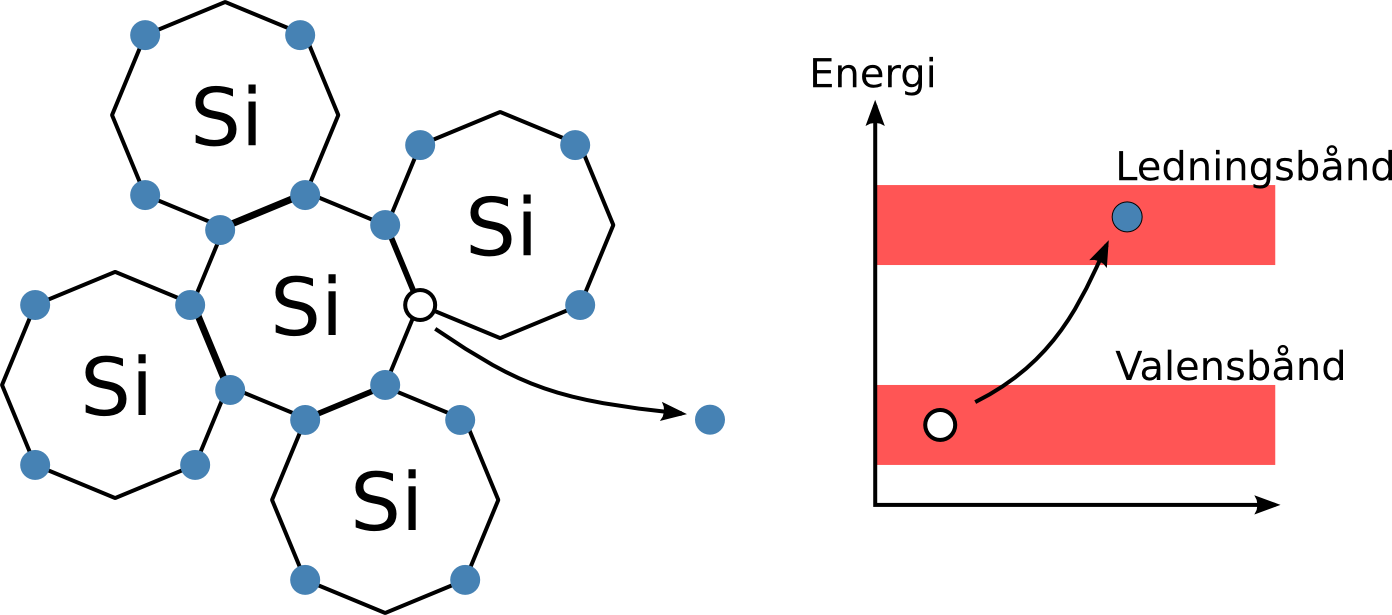
\includegraphics[width=\textwidth]{./img/krystall-ledning.png}
\\
Når elektroner faller tilbake igjen, ned i disse hullene,
kalles des rekombinasjon.


\subsection{Doping}
Hvordan doping fungerer er beskrevet i tidligere seksjoner.

\subsubsection{Pentavalent}
Pentavalente grunnstoffer (n-type) har 5 valenselektroner.
Dette gir et overflødig elektron som er svakt bundet.
Husk, stoffet er fremdeles nøytralt!
I denne type doping er elektronene majoritetsbærere.
\\\\
Eksempel:\\
P - fosfor\\
As - Arsenikk\\
Sb - Antimov\\
Bi - Bismut

\subsubsection{Trivalent}
Trivalente grunnstoffer (p-type) har 3 valenselektroner.
Vi får et hull blandt kovalentbindingene.
Elektroner er minoritetsbærere.
\\\\
Eksempel:\\
B - Bor\\
Al - Aluminium\\
Ga - Gallium\\
In - Indium


\subsection{PN-Junction}
Forklaring m/illustrasjon
Diffusjon
Forward bias
Reverse bias
TODO

\subsection{Dioder}
Forklaring, symbol etc
Ideell karakteristikk
Bulk resistans
Diode identifikasjon
TODO


  \section{Uke 7 - Bipolar Junction Transistorer (BJT)}
    Kap. 19, s. 617-652
+ notater på nett

\subsection{Oppbygning}
En bipolar junction transistor bruker både elektron- og hullstrøm,
og har 2 \emph{junctions} mellom ulikt dopede halvledere.
BJTer kommer i 2 typer, NPN og PNP. Vi skal se på den første av dem.

\paragraph{Collector, Base og Emittor} \mbox{} \\
En BJT består av 3 deler: collector, base og emittor.
Disse er bygget opp av tre dopede halvleder materialer, n-type og p-type.
Mellom disse regionene er pn-overganger akkurat som i dioder. \\\\
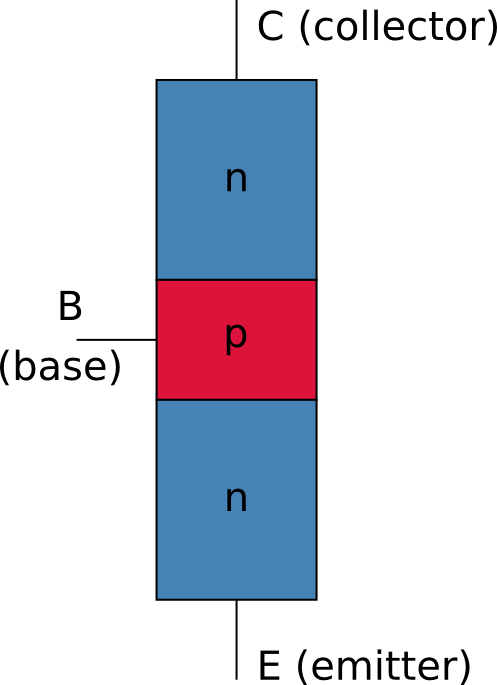
\includegraphics[width=0.5\textwidth]{./img/npn}
\\\\
Symbolet for BJTer ser slik ut for npn \\\\
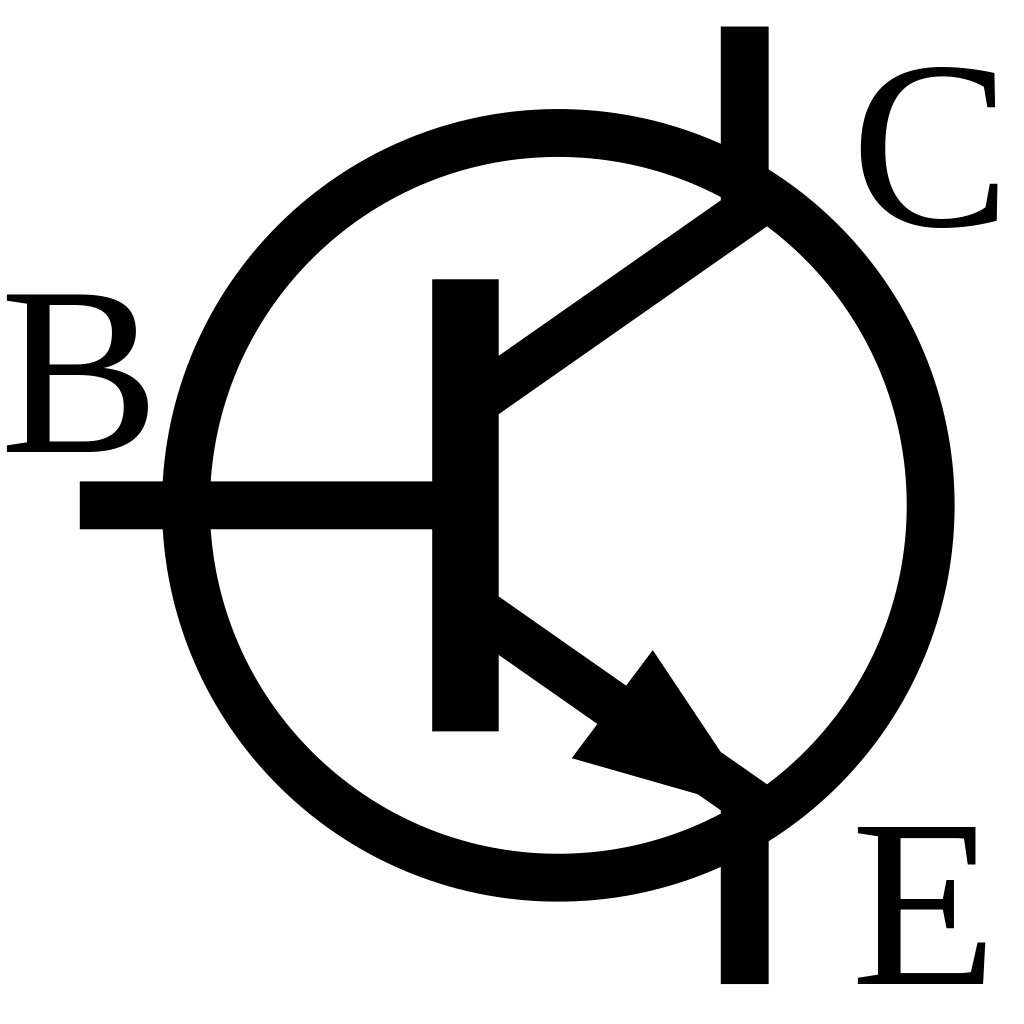
\includegraphics[width=0.25\textwidth]{./img/npn-symbol} \\
Hvor den lille pilen peker mot det n-dopede materialet.
\\
Tilsvarende for pnp \\\\
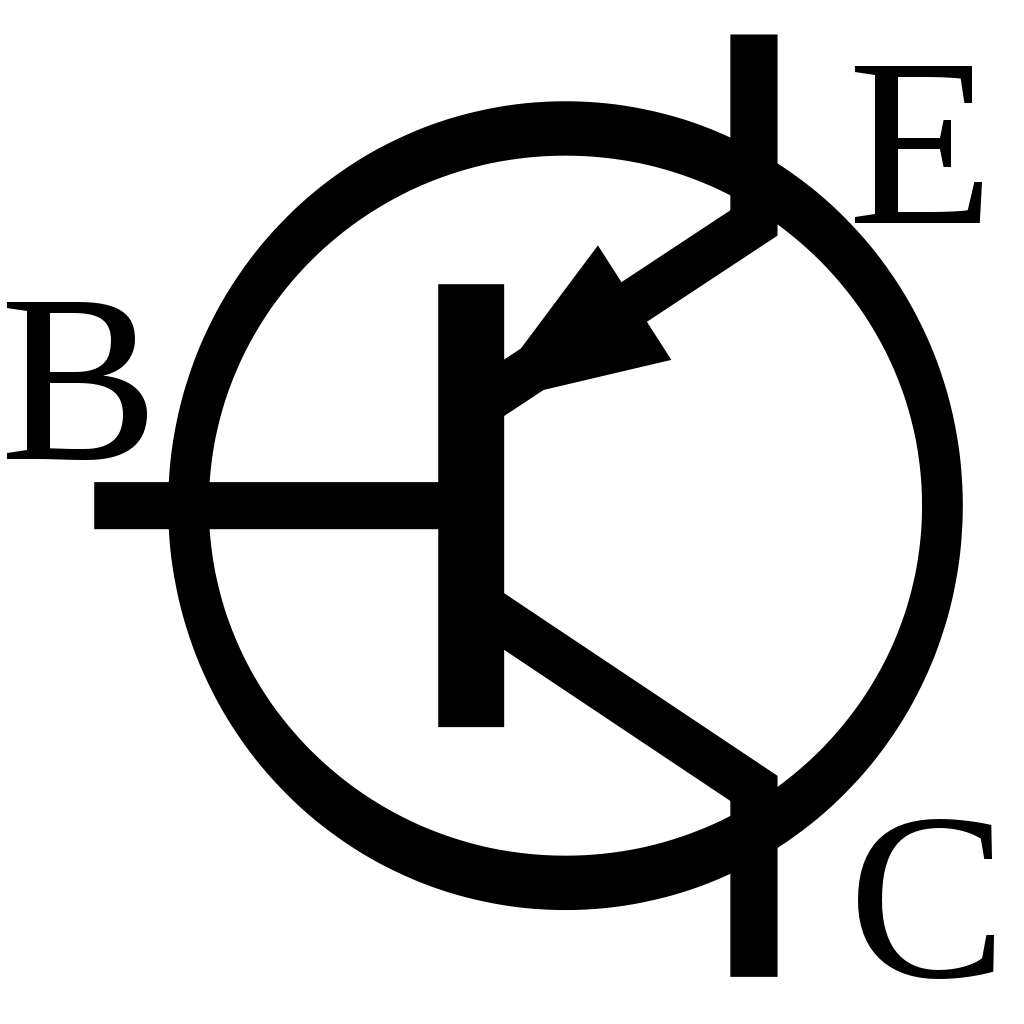
\includegraphics[width=0.25\textwidth]{./img/pnp-symbol}


\paragraph{Fysisk struktur} \mbox{} \\
I virkeligheten er en BJT bygget opp lag på lag med en isolator rundt.
\\\\
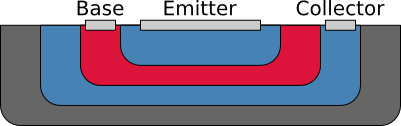
\includegraphics{./img/npn-real}


\subsection{Virkemåte}
  \subsubsection{Operasjonsmodi}
    Siden NPN-transistoren består av 2 PN-overganger,
kan man anse det som to dioder koblet sammen.
\\\\
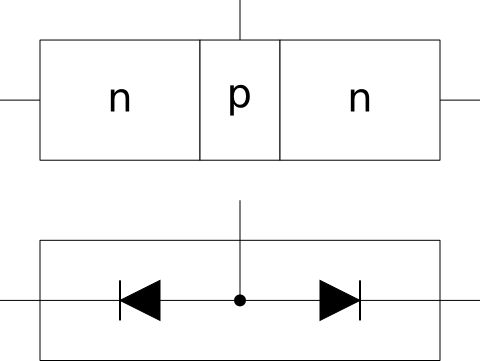
\includegraphics[width=0.5\textwidth]{./img/npn-bias}
\\\\
Disse diodene kan kjøres i forskjellig bias (forward, reverse).
Avhengig av forholdet mellom spenningen
ved diodens collector, base og emitter, fungerer transistoren forskjellig.

De forskjellige kombinasjonene utgjør transistorens operasjonsmodi.
\\\\
\begin{tabular}{ l | c | r}
Base-Emitter & Base-Collector & Operasjonsmodi \\ \hline
Reverse & Reverse & Cutoff \\
Forward & Reverse & Aktiv \\
Forward & Forward & Metning \\
\end{tabular}

  \subsubsection{Cutoff modus}
    Både base-emitter junction og collector-base junction
er i reverse bias.
Vi vet fra hvordan dioder fungerer at sperresjiktet
mellom de dopede materialene vokser.
I cutoff modus fungerer transistoren som en åpen krets,
ingen strøm passerer gjennom.
\\\\
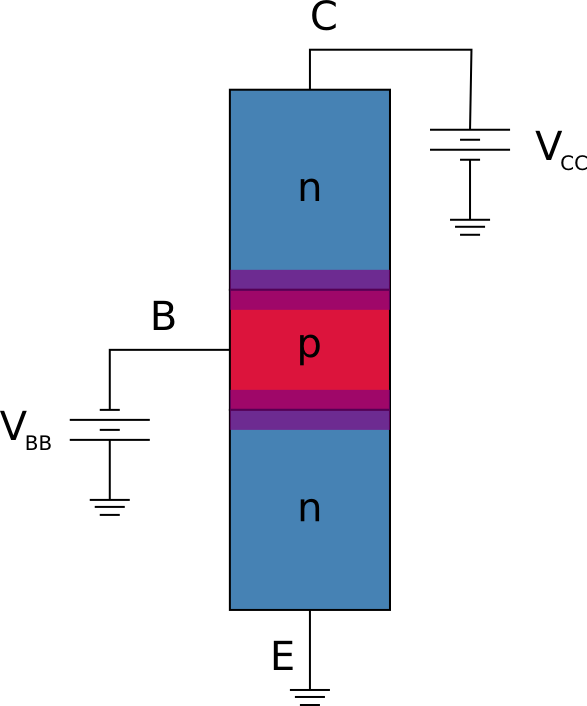
\includegraphics[width=0.5\textwidth]{./img/npn-cutoff}

  \subsubsection{Metning}
    Når spenningen ved basen er større enn ved collector,
fungerer transistoren som en kortslutning.
Strøm går fra emitter til collector.
\\\\
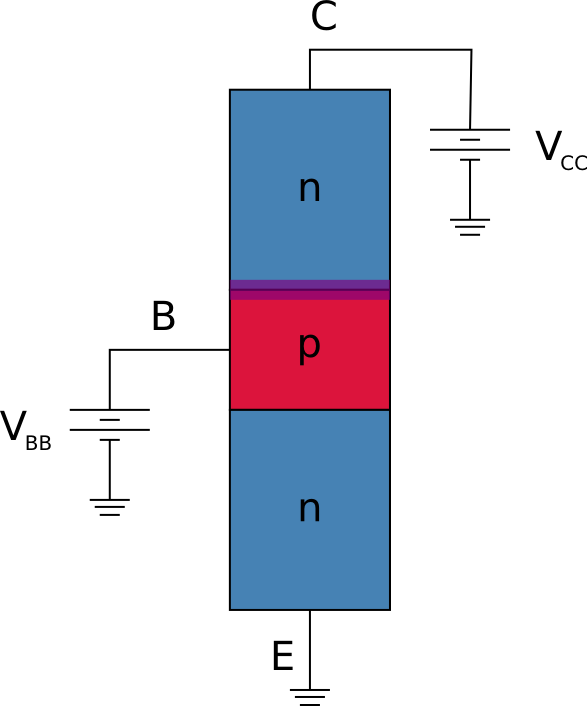
\includegraphics[width=0.5\textwidth]{./img/npn-metning}

  \subsubsection{Aktiv}
    Aktiv modus ser lik ut som ved metning, men med en forskjell.
Spenningen ved collector er større enn ved base.
$$V_C > V_B > V_E$$
I aktiv modus er strømmen fra emitter til collector
proporsjonal med strømmen til base.

  \subsubsection{Modi-kvadrant}
    En annen måte å illustrere transistorens modi på
er ved forholdet mellom spenningene.
\\\\
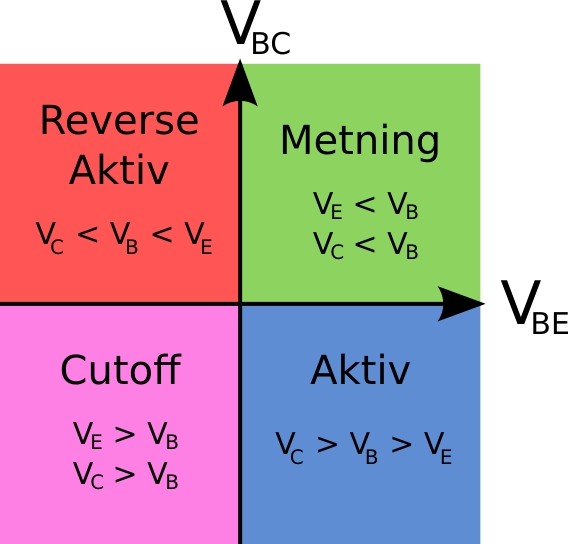
\includegraphics[width=0.5\textwidth]{./img/modi-kvadrant}
\\\\
$V_C = $ spenning fra collector til jord. \\
$V_E = $ spenning fra emitter til jord. \\
$V_B = $ spenning fra base til jord. \\
$V_{BC} = $ spenning fra base til collector. \\
$V_{BE} = $ spenning fra base til emitter. \\


\subsection{Karakteristikk}
  \subsubsection{Strøm}
    TODO

  \subsubsection{Virkeområde}
    TODO



  \section{Uke 8 - Transistorforsterkere og småsignalmodeller}
    Kap. 20, s 662 -695

\subsection{Universal Bias}
Her har det vært mye uklarheter.


Vi er blitt fortalt at det norske ordet
for universal bias er spenningsfordeler.
Etter å ha sett på flere kilder ser det ut til at
spenningsfordeling er noe som skjer, og må tas hensyn til,
under universal bias stabilization.

Formålet med universal bias stabilization, er å få et
stabilt Q-punkt (forklart straks).
Dette er bra for å få en gjevn $I_C$ uavhengig av $\beta$.

\subsubsection{Lastlinje}
Lastlinjen viser alle \emph{mulige} kombinasjoner av $I_C$ og $V_{CE}$.

For å ta hensyn til temperaturforandringer og andre forstyrrelser,
velger vi et punkt midt på denne linja.
\\\\
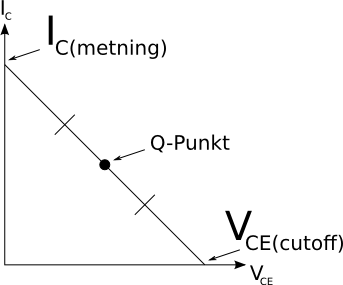
\includegraphics[width=0.5\textwidth]{./img/lastlinje}
\\\\
$$I_{C(metning)} = \frac{V_{CC}}{R_C}$$
$$V_{CE(cutoff)} = V_{cc}$$
Man bruker dette når man velger hvor store motstandere man vil ha.
$$R_C = \frac{V_{CE}}{I_C}$$



\subsection{Småsignalmodellen}
Småsignalmodellen brukes til å se hvordan en transistor
reagerer på små signaler ved å dele transistoren i to deler.
En dynamisk motstand $r_\pi$ mellom base-emitter.
Og en strømgenerator mellom collector-emitter.
Strømgeneratorens strøm bestemmes av transistorens
transkonduktans $g_m$ (steilhet).
\\\\
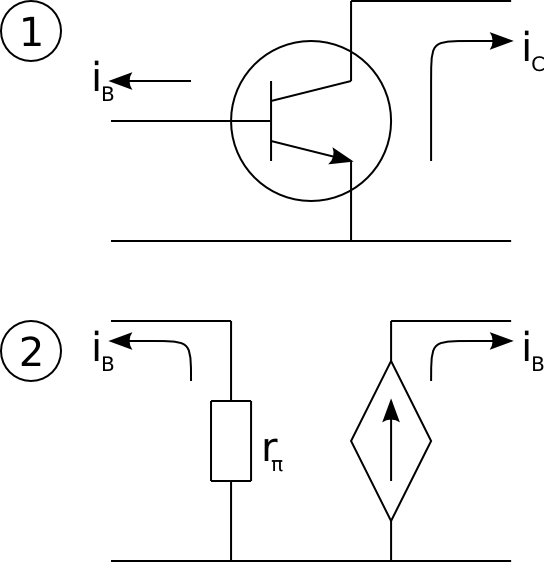
\includegraphics[width=0.5\textwidth]{./img/smasignal}
\\\\
$$i_C = \beta \cdot i_B$$
$$i_C = g_m \cdot V_{BE}$$

\subsubsection{Steilhet}
Transkonduktans?
TODO

\subsubsection{Dynamisk inngangsresistans}
TODO


\subsection{Spenningsforsterkning}
TODO



  \section{Uke 9}
  \section{Uke 10}
  \section{Uke 11}
  \section{Uke 12}
  \section{Uke 13}
  \section{Uke 14}
  \section{Uke 15}
  \section{Uke 16}
  \section{Uke 17}
  \section{Uke 18}
  \section{Uke 19}
  \section{Uke 20}
  \section{Uke 21}
  \section{Uke 22}
  \section{Uke 23}
\end{document}
